\documentclass{article}

\usepackage[T2A]{fontenc} % Кодировка шрифта
\usepackage[utf8]{inputenc} % Кодировка ввода
\usepackage[english,russian]{babel} % Языковые настройки
\usepackage{graphicx} % Для вставки изображений
\usepackage{amsmath} % Для использования математических формул
\usepackage{amsfonts} % Для использования математических символов и шрифтов
\usepackage{titlesec} % Для настройки заголовков разделов
\usepackage{titling} % Для настройки титульной страницы
\usepackage{geometry} % Для настройки размеров страницы

% Настройка заголовков разделов
\titleformat{\section}
  {\normalfont\Large\bfseries}{\thesection}{1em}{}
\titleformat{\subsection}
  {\normalfont\large\bfseries}{\thesubsection}{1em}{}

% Настройка титульной страницы
\setlength{\droptitle}{-4em} % Отступ заголовка
\title{\vspace{10cm}Задачи для самостоятельной работы по теории
вероятности}
\author{Вершинин Данил Алексеевич}
\date{Группа: Б9122-01-03-02мкт, Email: vershinin.da@dvfu.ru}

% Настройка размеров страницы
\geometry{a4paper, margin=2cm}

\begin{document}
\maketitle
\newpage
\section*{Задача №1}
\subsection*{Условие}
Шестигранная игральная кость устроена таким образом, что у любого
четного числа в два раза больше шансов выпасть, чем у нечётного. Все четные
стороны равновероятны ровно так же, как и нечётные. Постройте вероятностную
модель в которой кость бросается один раз и найдите вероятность того, что выпадет
число меньше чем 4. 
\subsection*{Решение}
Всего у нас 6 вариантов исходов при бросании игральной кости. При чём вероятность выпадения четного числа в 2 раза выше, чем нечетного. Обозначим за $n$ вероятность выпадения нечетного числа. Тогда вероятность выпадения чётного равна $2n$. Три варианта выпадения нечетного числа и столько же четного. Суммируем и получаем $3n + 6n = 9n$. При этом, сумма всех вероятностей должна равняться единице. Отсюда получаем:
\[
    9n = 1 \ \Rightarrow \ n = \frac{1}{9}
\]
Следовательно, вероятность выпадения нечетного числа равна $\frac{1}{9}$. Тогда вероятность выпадения четного числа равна $\frac{2}{9}$. \\
Построим вероятностную модель:\\
\begin{figure}[h]
    \centering
    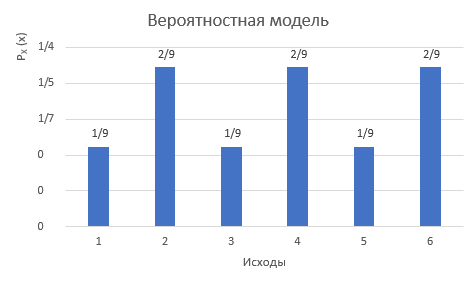
\includegraphics[width=0.75\textwidth]{1.png}
    \caption{Вероятностная модель}
    \label{fig:prob_dia}
\end{figure}\\
Вероятностью выпадения числа, меньшего чем 4, является сумма вероятностей исходов, удовлетворяющих условию (x < 4).
\[
    P(X| x < 4) = \frac{1}{9} + \frac{2}{9} + \frac{1}{9} = \frac{4}{9}
\]
\subsection*{Ответ}
Рис. 1, $\frac{4}{9}$
\newpage
\section*{Задача №2}
\subsection*{Условие}
Четырехгранная игральная кость бросается последовательно до тех пор,
пока не выпадет четное число (если такое событие наступит). Каково множество
исходов у этого эксперимента?
\subsection*{Решение}
При бросании четырёхгранной кости четыре исхода $\{ 1, 2, 3, 4\}$. Обозначим за $A$ - событие, при котором выпадает нечетные числа (1, 3), а за $B$ - выподение четных числе (2, 4).\\
Таким образом, всевозможные исходы этого эксперимента можно записать следующим образом:
\[
    \Omega = \{B, AB, AAB, \dots \}
\]
\subsection*{Ответ}
$\Omega = \{B, AB, AAB, \dots \}$
\section*{Задача №3}
\subsection*{Условие}
Вы участвуете в турнире по шахматам из четырех претендентов в котором
играете одну игру каждым участником. Зная вероятность своей победы в каждой
партии, вы можете выбирать в каком порядке играть с каждым участником. Победа в
турнире отдаётся игроку, который победил в двух партиях подряд. Вы можете играть
вторую партию со слабейшим игроком или играть партии с оставшимися двумя
игроками в произвольном порядке. В каком случае у вас будут максимальные шансы
на победу? 
\subsection*{Решение}
Пусть вероятности победы над каждым соперником соответсвенно равны $A, B, C$. Пусть первый наш противник будет тот, вероятность побуды над которым равна $A$. Также условимся, что слабейшим из оставшихся двух будет тот, вероятность победы над которым равна $B$. Рассмотрим неравенство:
\[
    C < B
\] 
Теперь найдём вероятности проигрыша в каждой партии и построим неравенство:
\[
    (1 - B) < (1 - C)
\] 
Перемножив соответсвующие части получим:
\[
    C(1 - B) < B(1 - C) \ (*)
\]
Рассмотрим полную вероятность победы:
\[
    P(W) = ABC + (1 - A) BC + ( \max(AB(1-C), AC(1-B) ) \overset{(*)}{=} ABC + (1 - A) BC + AB(1-C)
\]
$\max(AB(1-C), AC(1-B)$ - в данном случае выступает в качестве условия на выбор второго соперника. А т.к. наша задача получить наилучшие шансы на победу, мы должны выбрать самое большое из предлагаемых слагаемых.
\subsection*{Ответ}
Максимальные шансы на победу будут в том случае, если выбрать слабейшего соперника из оставшихся.

\section*{Задача №4}
\subsection*{Условие}
Шестигранная игральная кость бросается дважды. Все 36 исходов
равновероятны. Найдите вероятность выпадения дубля. Зная, что сумма выпавших
костей меньше либо равна четырем, найдите условную вероятность дублей. Найдите
вероятность, что хотя бы на одной кости выпала 6. Зная, что на всех костях выпали
разные числа, найдите вероятность того, что хотя бы на одной из них выпала 6.  
\subsection*{Решение}
Выпадение дубля.\\
Могут выпасть следующие дубли: $\{ (1,1), (2,2), (3,3), (4,4), (5,5), (6,6) \}(*)$, количество реализаций равно 6. Всего исходов 36. Отсюда, вероятность выподения дубля равна $P(x) = \frac{n}{m}=\frac{6}{36} = \frac{1}{6}$.\\
\\
Условная вероятность выпадения дубля, при условии, что сумма меньше или равна четырём.\\
Пусть $A$ - вероятность выпадения дубля, а $B$ - вероятность того, что сумма чисел при двух бросках меньше или равна четырём. Всего условий, удовлетворяющих условию (сумма меньше или равна четырём) 6: $B=\{ (1,1), (1,2), (1,3), (2,1), (2,2), (3,1)\}; \ |B| = 6$.\\
При этом, вероятность выпадения дубля, при условии, что сумма результатов меньше или равна четырём равна $P(A \cap B) = \frac{n}{m} = \frac{2}{36}$.\\
Тогда по формуле условной вероятности получаем:\\
\[
    P(A|B) = \frac{P(A \cap B)}{P(B)} = \frac{2}{36} \times \frac{6}{1} = \frac{2}{6} = \frac{1}{3}
\]\\
\\
Выпала хотя бы одна 6-ка.\\
Количство всех вариантов обозначим за $m = 36$.\\
Количество вариантов, при котрых выпадает хотя бы одна 6, обозначим за $n$:\\ $A =\{ (6, 1), (6, 2), (6, 3), (6, 4), (6, 5), (1, 6), (2, 6), (3,6), (4, 6), (5,6), (6,6) \ n = |A| = 11\}$.
Отсюда найдём вероятность события, которое удовлетворяет всем условиям: $P(X) = \frac{n}{m} = \frac{11}{36}$ \\
\\
Выпала хотябы одна 6-ка, при условии выпадений без дубля.\\
Всего вариантов, которые удовлетворяют условию буз дублей, обозначим за $m = 36 - 6 = 30$. (т.к. мы исключаем все дубли (*)). И всего вариантов, при которых выпалала 6 без дублей, обозначим за $n$: $A = \{  (6, 1), (6, 2), (6, 3), (6, 4), (6, 5), (1, 6), (2, 6), (3,6), (4, 6), (5,6), \ n = |A| = 10\}$.\\
Отсюда найдём вероятность события, которое удовлетворяет всем условиям: $P(X) = \frac{n}{m} = \frac{10}{30} = \frac{1}{3}$ 
\subsection*{Ответ}
$\frac{1}{6}$, $\frac{1}{3}$, $\frac{11}{36}$, $\frac{1}{3}$,
\section*{Задача №5}
\subsection*{Условие}
Монета подбрасывается дважды. Верно ли утверждение, что вероятность
выпадения двух орлов более вероятно, если будет известно, что первая монета
выпала орлом, чем то что хотя бы одна монета выпала орлом? Зависит ли это от
смещения монеты? 
\subsection*{Решение}
Обозначим за $A$ - событие, при котором орёл выпадает при первом броске. За $B$ - событие, когда орёл выпадает при втором броске. Будем считать, что вероятность выпадения орла $p$, тогда вероятность выпадения решки $1-p$. События $A$ и $B$ независимы. \\
Тогда, вероятность события "два орла" при условии, что первый бросок был орёл, равна:\\
\[
    P(A \cap B|A) = \frac{P(A\cap B)}{P(A)} = \frac{p^2}{p} = p 
\]\\
Вероятность события "два орла", при условии, что при броске монеты выпал орел, равна:\\
\[
    P(A \cap B| A \cup B) = \frac{P(A \cap B)}{P(A \cup B)} = \frac{p^2}{2p} = \frac{p}{2}
\]\\
Можнос делать вывод о том, что вероятность первого события выше, чем второго. Следовательно, утверждение верно. При этом результат не зависит от смещения. 
\subsection*{Ответ}
Утверждение верно. От смещения не зависит.
\section*{Задача №6}
\subsection*{Условие}
Дано три монеты. Две монеты имеют орлов на обоих сторонах, одна монета
имеет орла на одной стороне и решку на другой. Одна монета выбирается случайно и
подбрасывается. Зная что выпал орел, какая вероятность того, что обратная сторона
будет решкой?
\subsection*{Решение}
Для решения этой задачи необходимо применить привило Баеса. Т.е. необходимо взять вероятность того, что мы выбрали обычную монету (обозначим за $A$) и выпал орёл, и поделить её на сумму вероятностей того, что выпал орёл(обозначим за B).\\
\[
    P_X(A|B) = \frac{P(A \cap B)}{P(B)} = \frac{P(A) \times P(B|A)}{\sum_i P(A_i)\times P(B|A_i)} = \frac{\frac{1}{3}\times\frac{1}{2}}{\frac{1}{3} \times 1 + \frac{1}{3} \times 1 + \frac{1}{3}\times\frac{1}{2}} = (*)
\]
\[
    (*) = \frac{\frac{1}{6}}{\frac{2}{3} + \frac{1}{6}} = \frac{1}{6} \times \frac{6}{5} = \frac{1}{5}
\]
Выше, $A_i$ - это вероятность выбора монеты.
Таким образом, мы получили вероятность того, что выбранная монета обычная, следовательно обратная сторона является решкой
\subsection*{Ответ}
$\frac{1}{5}$
\section*{Задача №7}
\subsection*{Условие}
На заводе проводится контроль качества изготовленных деталей. Из ста
деталей случайно выбираются четыре. Если хотя бы одна деталь бракованная, вся
партия не проходит контроль. Какова вероятность того, что партия пройдет контроль,
если из ста деталей пять бракованных? 
\subsection*{Решение}
Для решения этой задачи нужно найти количество вариантов того, что выберут именно те детали, которые пройдут контроль качества; и поделить на общее количество вариантов выборки.\\
Количество вариантов выбора качественной детали обозначим за $n = \binom{95}{4}$ (из ста деталей 5 - бракованные, итого качественных 95, а выбирают 4).\\
Количество всех вариантов выборки обозначим за $m = \binom{100}{4}$\\
Таким образом, получаем вероятность того, что партия пройдёт проверку:\\
\[
    P(X) = \frac{n}{m} = \frac{\binom{95}{4}}{\binom{100}{4}} \approx 0.81
\]
\subsection*{Ответ}
$\frac{\binom{95}{4}}{\binom{100}{4}} \approx 0.81$
\section*{Задача №8}
\subsection*{Условие}
Докажите, что \(P(A \cap B\mid B) = P(A\mid B)\).
\subsection*{Решение}
По определению:
\[
    P(A\cap B|B) \iff \frac{P((A\cap B) \cap B)}{P(B)} \iff \frac{P(A \cap B)}{P(B)} \iff P(A|B)
\]
\subsection*{Ответ}
Доказано
\section*{Задача №9}
\subsection*{Условие}
Представьте, что вы сдаёте положительный тест на редкую болезнь
(вероятность заболеть 1\%). Глядя в инструкцию, вы обнаруживаете, что тест
показывает положительный результат, при том, что пациент действительно болен, с
вероятностью 99\%. Если пациент не болен, то тест ошибочно показывает
положительный результат только в 5\% случаев. Какова вероятность, что вы
действительно больны, если тест показывает положительный результат?
\subsection*{Решение}
Для решения этой задачи удобно использовать правило Баеса.
Обозначим за $A$ - вероятность того, что пациент действительно болен. Вероятность этого равна 0.01, а вероятность противоположного события $A^c = 1-0.01 = 0.99$.\\
$B$ - вероятность того, что тест сработает. Вероятность равна 0.95, а вероятность противоположного события $B^c = 1 - 0.95 = 0.05$.\\
Тогда, решение сводится к следующему:\\
\[
    P(A|B) = \frac{P(A \cap B)}{\sum_i P(A_i)\times P(B|A_i)} = \frac{0.01 \times 0.99}{0.01\times 0.99 + 0.99 \times 0.05} = \frac{1}{6}
\]
\subsection*{Ответ}
$\frac{1}{6}$
\section*{Задача №10}
\subsection*{Условие}
Допустим $n$ человек прибывают на вечеринку. Какова вероятность того, что
каждый из них имеет различный день рождения? (Для простоты исключите
перекрывающиеся события, например, 29 февраля). 
\subsection*{Решение}
Всего различных дней 365. Тогда, первый, что приходит на вечеринку гарантированно с уникальным днём рождения. Второй имеет вероятность $\frac{364}{365}$, третий - $\frac{363}{365}$ и так далее. Это будет верно для $1\le n \le 365 $. Если n > n - вероятность равна нулю\\
Формализуем решение:
\[
    1 \times \frac{364}{365} \times \frac{363}{365} \times \dots \times \frac{365 - n + 1}{365} = \frac{365!}{(365 - n)! \times 365^n}
\]
\subsection*{Ответ}
$\begin{cases}
    \frac{365!}{(365 - n)! \times 365^n}, \ n \le 365 \\
    0, \ \text{otherwise}
\end{cases}$

\section*{Задача №11}
\subsection*{Условие}
Из колоды в 52 карты раздаётся 13 карт. Найдите вероятность того, 13
карта в раздаче будет первым королём из колоды. Все исходы равновероятны. 
\subsection*{Решение}
В колоде 52 карты. Из них 4 короля. Вероятность вытащить первую  карту, которая не является королём равно $P(X_1)=\frac{48}{52}$, вторую - $P(X_2)=\frac{47}{51}$, и так далее. На двенадцатой карте получим $P(X_{12})=\frac{37}{41}$. Тринадцатой картой нам нужно вытянуть короля: 4 короля всё ещё в колоде, а карт осталось 40. Отсюда $P(X_{13})=\frac{4}{40}$.
Приведём к математическим выкладкам:
\[
    \frac{48}{52} \times \frac{47}{51} \times \dots \times \frac{37}{41} \times \frac{4}{40} = \frac{48!}{36!}\times\frac{40!}{52!}\times\frac{4}{40} = \frac{703}{20825} \approx 0.03
\]
\subsection*{Ответ}
$\frac{703}{20825} \approx 0.03$
\section*{Задача №12}
\subsection*{Условие}
Футбольная команда играет недельный турнир из двух игр. Вероятность не
проиграть в первой игре равна 0,4, не проиграть во второй игре 0,7. Если команда не
проиграла в игре, то вероятность победы равновероятна (либо победа либо ничья). За
проигрыш команде не начисляются очки, за ничью полагается 1 очко, за победу – 2.
Простройте функцию вероятности для количества набранных очков, которые команда
получит по итогам турнира. 
\subsection*{Решение}
Пусть событие "не проиграть первую игру"  $=A$, $P(A) = 0.4$, следовательно, вероятность проигрыша $P(\overline{A}) = 1 - P(A) = 1 - 0.4 = 0.6$. Вероятность победы в первой игре равно вероятности ничьей в первой игре и равно половине вероятности непроигрыша: $P(A_W) = P(A_T) = P(A) / 2 = 0.2$.
Проведём аналогичные рассуждения со второй игрой.\\
Событие $B$ - не проиграть вторую игру. Его вероятность $P(B) = 0.7$. Вероятность проигрыша - $P(\overline{B}) = 1 - P(B) = 0.3$. Вероятность победы равна вероятности ничьей и равна половине вероятности непроигранной игры: $P(B_W) = P(B_T) = P(B)/2 = 0.7/2 = 0.35$.\\
Все событие независимые.
Начнём вычисления:\\
0 очков: $P(k=0)=P(\overline{A}) \times P(\overline{B}) = 0.6 \times 0.3 = 0.18$\\
1 очко: $P(k=1) = P(A_T)\times P(\overline{B}) + P(\overline{A})\times P(B_T) = 0.2\times 0.3 + 0.6\times 0.35 = 0.27$\\
2 очка: $P(k=2)=P(A_W)\times P(\overline{B}) + P(A_T) \times P(B_T) + P(\overline{A})\times P(B_W) = 0.2\times 0.3 + 0.2\times 0.35 + 0.6\times 0.35 = 0.34$\\
3 очка: $P(k=3) = P(A_W)\times P(B_T) + P(A_T) \times P(B_W) = 0.2\times 0.35 + 0.2\times 0.35 = 0.14$\\
4 очка: $P(k=4) = P(A_W)\times P(B_W) = 0.2 \times 0.35 = 0.07$
\subsection*{Ответ}
\begin{center}
 \begin{tabular}{||c |c ||} 
 \hline
 k & $P_X(k)$  \\
 \hline
 0 & 0.18\\
 \hline
 1 & 0.27  \\ 
 \hline
 2 & 0.34  \\
 \hline
 3 & 0.14  \\
 \hline
 4 & 0.07  \\
 \hline
\end{tabular}
\end{center}

\section*{Задача №13}
\subsection*{Условие}
Ян Непомнящий и Магнус Карлсен играют тайбрейк из 10 игр на чемпионате
по шахматам. Вероятность победы Магнуса в конкретной игре равна 0,2, вероятность
победы Яна – 0,1 и вероятность ничьей равна 0,7. Если один из игроков выигрывает
игру, он выигрывает тайбрейк. Если все 10 игр завершаются ничейными партиями, то
тайбрейк объявляется ничейным. Найдите вероятность победы Яна. Постройте
функцию вероятности длительности тайбрейка. 
\subsection*{Решение}
В данной задаче необходимо использовать геометрическое распределение.
Для расчёта вероятности победы Яна необходимо посчитать сумму вероятностей победы Яна в каждом раунде тайбрейка: \\$\sum\limits_{n=1}^{10}0.7^{n-1}0.1\approx 0.32$\\
Для расчёта функции вероятности продолжительности необходимо учесть, что при каждом раунде возможны два исхода: ничья с вероятностью 0.7 или победа одного из участников тайбрейка - 0.3. Т.к. вероятность наступления победы одного из участников в следующем напрямую зависит от результатов предыдущих партий, то в данном случае ($x \in [1, 10]$) как раз следует использовать геометрическое распределение:\\
\[
    P_X(x) = 0.7^{x-1}0.3 + {\lfloor \frac{x}{10} \rfloor}0.7^{x}
\]\\
x в данном случае является количеством раундов тайбрейка.\\
Первое слагаемое представляет ситуацию, когда тайбрейк заканчивается победой одного из участников. Второе же, является вероятностью того, что тайбрейк закончится ничьей. При $x \in [1, 9]$ оно будет равно 0 и не повлияет на результат.
\subsection*{Ответ}
$\sum\limits_{n=1}^{10}0.7^{n-1}0.1\approx 0.32$, $P_X(x) = \begin{cases}
    0.7^{x-1}0.3 + {\lfloor \frac{x}{10} \rfloor}0.7^{x}& x \in [1, 10]\\
    0& \text{otherwise}
\end{cases}$
\section*{Задача №14}
\subsection*{Условие}
Вы купили большой дом. При покупке реэлтор дал вам пять ключей от
разных дверей в доме, которые выглядят примерно одинаково. Вы хотите открыть
входную дверь. Постройте функцию вероятности для попыток открыть дверь в двух
вариантах: 1. Вы пробуете один ключ и не используете его в последующих попытках;
2. Вы кладёте использованный ключ обратно и можете потенциально выбрать его
снова. 
\subsection*{Решение}
1) Изначально у нас имеется 5 ключей. Следовательно, вероятность открыть дверь с первого раза равна $\frac{1}{5}$.\\
Вторая попытка предполагает, что первая увенчалась неудачей и неподходящий ключ убран из выборки.
\[
    P(2) = (1-\frac{1}{5})\times \frac{1}{4} = \frac{4}{5} \times \frac{1}{4} = \frac{1}{5}
\]
Такую же логику можем применить к вариантам, когда мы открываем дверь с третьего, четвертого и пятого раза. Нетрудно заметить, что вероятность каждого случая равна $\frac{1}{5}$.
Таким образом, функция вероятности в данном случае равна:
\[
    P_X(K) = \frac{1}{5}
\]
2) В данном случае воспользуемся геометрическим распределением. Так как количество ключей в саппорте - значение постоянное и верным является только один, получим что вероятность того, что ключ подходит равна: $p = \frac{1}{5}$. В тоже время вероятность ошибки в  выборе: $1-p = \frac{4}{5}$.\\
Отсюда получаем, что функция вероятности для данного случая равна:
\[
    P_X(k) = \biggl(\frac{4}{5}\biggr)^{k-1}\times\frac{1}{5}
\]
\subsection*{Ответ}
$P_X(K) = \frac{1}{5}; \     P_X(k) = \biggl(\frac{4}{5}\biggr)^{k-1}\times\frac{1}{5}$
\section*{Задача №15}
\subsection*{Условие}
В футбольную команду из 10 игроков принимают двух нападающих. Каждый
из 10 игроков в отдельности может равновероятно быть нападающим. Постройте
функцию вероятности количества нападающих в новой команде 
\subsection*{Решение}
Введём случайную величину $X$ - количество нападающих в команде. Все 10 игроков различны и нас интересует выборка из них. Поэтому будем использовать биноминальное распределение. Вероятность каждого попасть в команду, в качестве нападающего, равна $p = \frac{1}{10}$. Отсюда, вероятность обратного события равна: $q=1 - \frac{1}{10} = \frac{9}{10}$. Получим формулу:
\[
    P(X=k) = \binom{10}{k}p^kq^{10-k} = \binom{10}{k}0.1^k0.9^{10-k}
\]
Но в условии задачи написано, что двое из них, гарантированно попадут в команду. Слдовательно, необходимо, чтобы функци при $k \in [1,2]$ равнялась 1.
Получим:
\[
    P_X(x) = \begin{cases}
        1, & x \leq 2 \\ 
        \binom{10}{x} \cdot 0.1^{x} \cdot 0.9^{10-x}, & \text{otherwise } \end{cases}
\]
\subsection*{Ответ}
$P_X(x) = \begin{cases}
    1, & x \leq 2 \\ 
    \binom{10}{x} \cdot 0.1^{x} \cdot 0.9^{10-x}, & \text{otherwise } \end{cases}
    $

\section*{Задача №16}
\subsection*{Условие}
Пусть задана случайная величина X следующей функцией вероятности: \(P_X(x) = \frac{x^2}{a}\), если \(x \in [-3, 3]\), \(\quad p_X(x) = 0\) – в других случаях. Найдите математическое
ожидание $X$ . Найдите функцию вероятности для \(Z = (X - E[X])^2\). Используя \(Z\) найдите дисперсию \(X\).
\subsection*{Решение}
Для нахождения математического ожидания, сначала нужно определить константу \(a\). Поскольку \(P_X(x)\) является функцией вероятности, сумма вероятностей по всем возможным значениям \(X\) должна быть равна 1:

\[ \sum_{x=-3}^{3} P_X(x) = \sum_{x=-3}^{3} \frac{x^2}{a} = 1 \]

Вычислим сумму:

\[ \sum_{x=-3}^{3} x^2 = (-3)^2 + (-2)^2 + (-1)^2 + 0^2 + 1^2 + 2^2 + 3^2 = 9 + 4 + 1 + 0 + 1 + 4 + 9 = 28 \]

Теперь мы можем найти \(a\):

\[ \frac{28}{a} = 1 \Rightarrow a = 28 \]

Теперь, когда мы знаем \(a\), мы можем найти математическое ожидание \(E[X]\):

\[ E[X] = \sum_{x=-3}^{3} x \cdot P_X(x) = \sum_{x=-3}^{3} x \cdot \frac{x^2}{28} \]

Поскольку функция \(x \cdot \frac{x^2}{28}\) является нечетной (\(f(-x) = -f(x)\)), сумма по симметричному интервалу от -3 до 3 будет равна нулю:

\[ E[X] = 0 \]

Теперь, когда мы знаем, что \(E[X] = 0\), мы можем найти функцию вероятности для \(Z = (X - E[X])^2\):

\[ Z = X^2 \]

Так как \(E[X] = 0\), функция вероятности \(Z\) будет такой же, как и \(X^2\), но с учетом того, что \(X\) принимает значения от -3 до 3:

\[ P_Z(z) = P_X(\sqrt{z})  = \frac{z}{a} = \frac{z}{28}\]

Теперь мы можем использовать \(Z\) для нахождения дисперсии \(X\):

\[ \text{Var}(X) = E[Z] = E[X^2] = \sum_{x=-3}^{3} x^2 \cdot P_X(x) = \sum_{x=-3}^{3} \frac{x^4}{28} \]

Вычислим сумму:

\[ \text{Var}(X) = \frac{1}{28} \left((-3)^4 + (-2)^4 + (-1)^4 + 0^4 + 1^4 + 2^4 + 3^4\right) \]
\[ \text{Var}(X) = \frac{1}{28} \left(81 + 16 + 1 + 0 + 1 + 16 + 81\right) \]
\[ \text{Var}(X) = \frac{1}{28} \cdot 196 \]
\[ \text{Var}(X) = 7 \]

Таким образом, дисперсия \(X\) равна 7.
\subsection*{Ответ}
$0, \frac{z}{28}, 7$

\section*{Задача №17}
\subsection*{Условие}
Предположим, что шестигранную кость бросают 4 раза, все исходы
равновероятны. Пусть \(X\) это число выпавших единиц, а \(Y\) чисто выпавших двоек.
Постройте совместную функцию вероятности для \(X\) и \(Y\). 
\subsection*{Решение}
Для построения совместной функции вероятности для X и Y, где X - количество выпавших единиц, а Y - количество выпавших двоек, мы можем воспользоваться мультиномиальным распределением, так как у нас несколько категорий исходов (в данном случае, числа от 1 до 6 на шестигранных костях).

Формула мультиномиального распределения:
\[ P(X=x, Y=y) = \frac{n!}{x! \cdot y! \cdot (n-x-y)!} \cdot p_1^x \cdot p_2^y \cdot p_3^{n-x-y} \]

Где:


 n - общее количество бросков (4)


 x - количество выпавших единиц


 y - количество выпавших двоек


 $p_1, p_2, p_3$ - вероятности выпадения единицы, двойки и других чисел соответственно (в данном случае, 1/6 для каждого числа)

Таким образом, совместная функция вероятности для X и Y будет выглядеть следующим образом:
\[ P(X=x, Y=y) = \frac{4!}{x! \cdot y! \cdot (4-x-y)!} \cdot \left(\frac{1}{6}\right)^x \cdot \left(\frac{1}{6}\right)^y \cdot \left(\frac{4}{6}\right)^{4-x-y} \]

где x и y принимают значения от 0 до 4, так как количество выпавших единиц и двоек не может превышать общее количество бросков (4).
\subsection*{Ответ}
$P(X=x, Y=y) = \frac{4!}{x! \cdot y! \cdot (4-x-y)!} \cdot \left(\frac{1}{6}\right)^x \cdot \left(\frac{1}{6}\right)^y \cdot \left(\frac{4}{6}\right)^{4-x-y}$

\section*{Задача №18}
\subsection*{Условие}
Ваш путь до учебного корпуса ДВФУ имеет четыре светофора. На каждом
из них, не зависимо от другого, вы можете равновероятно встретить красный или
зелёный свет. Постройте функцию вероятности и рассчитайте математическое
ожидание для количества остановок на светофорах. В случае, если горит красный вы
ждёте две минуты. Рассчитайте дисперсию ожидания по пути на учёбу. 
\subsection*{Решение}
Положим, что $X$ - множество количества остановок на светофорах. Найдём вероятность для каждой реализации:\\
$0. \left(\frac{4}{0}\right) \times \frac{1}{16} = \frac{1}{16}$\\
$1. \left(\frac{4}{1}\right) \times \frac{1}{16} = \frac{4}{16}$\\
$2. \left(\frac{4}{2}\right) \times \frac{1}{16} = \frac{6}{16}$\\
$3. \left(\frac{4}{3}\right) \times \frac{1}{16} = \frac{4}{16}$\\
$4. \left(\frac{4}{4}\right) \times \frac{1}{16} = \frac{1}{16}$\\
Проверим на полноту: $\frac{1}{16} + \frac{4}{16} + \frac{6}{16} + \frac{4}{16} + \frac{1}{16} = 1$. Верно; следовательно, при объединении, эти события дают полную группу событий.\\
Отсюда, функция вероятности будет иметь следующую форму:
\[
    P_X(x)=\frac{\binom{4}{x}}{16}
\]
Найдём математическое ожидание:
\[
    E[X] = \sum_{x=0}^{4}x \times \frac{\binom{4}{x}}{16} = 0 + \frac{4}{16} + \frac{12}{16} + \frac{12}{16} + \frac{4}{16} = 2
\]
Теперь можно найти дисперсию ожидания по пути на учёбу. Учитывая, что на каждую остановку приходится по 2 минуты ожидания, то обозначим за $Y$ - множество количества минут, которые провели в ожидании зелёного сигнала светофора. Оно зависит от $X$ по правилу: $Y=2X$.
Отсюда, дисперсия равна:
\[
   Var(Y) = Var(2X)= 4 \times Var(X) = 4 \times \left(E[X^2] - (E[X])^2\right) = 4 \times \left(\sum_{x=0}^{4} x^2\frac{\binom{4}{x}}{16} - 4\right) =
\]
\[
    4 \times \left(0 + \frac{4}{16} + \frac{24}{16} + \frac{36}{16} + \frac{16}{16} - 4 \right) = 4 \times 1 = 4
\]
\subsection*{Ответ}
$F_X(x) = \frac{\binom{4}{x}}{16}, \ 2, \ 4 $

\section*{Задача №19}
\subsection*{Условие}
 Пусть X непрерывно равномерно распределённая величина на интервале
[0,1]. Пусть случайная величина Y имеет следующую функцию вероятности:
\(Y = g(X) = \begin{cases}
  1, & \text{если } x \leq \frac{1}{3} \\
  2, & \text{если } x > \frac{1}{3}
\end{cases}\) Найдите математическое ожидание Y. 
\subsection*{Решение}
Дано, что X - непрерывно равномерно распределённая величина, следовательно, что $P_X(x) = C$, где $C$ - константа, отсюда следует, что $F_X(x) = x $.
Теперь можно посчитать вероятность, воспользовавшись формулой $P(a\le x \le b) = F(b) - F(a)$. Далее, найдём вероятность для каждого случая:
\[
    P(x \le \frac{1}{3}) = F(\frac{1}{3}) - F(0) = \frac{1}{3} 
\]
\[
    P(X > \frac{1}{3}) = F(1) - F(\frac{1}{3}) = 1 - \frac{1}{3} = \frac{2}{3}
\]
Теперь можно найти математическое ожидание:
\[
    E[Y] = 1 \times P(x \le \frac{1}{3}) + 2 \times P(x > \frac{1}{3}) = 1 \times \frac{1}{3} + 2 \times \frac{2}{3} = \frac{5}{3}
\]
\subsection*{Ответ}
$E[Y] = \frac{5}{3}$
\section*{Задача №20}
\subsection*{Условие}
 ???
\subsection*{Решение}
\subsection*{Ответ}

\section*{Задача №21}
\subsection*{Условие}
Пусть \(Y = g(X) = X^2\), где случайная величина с известной функцией
плотности вероятности. Найдите плотность вероятности \(f_Y(y)\).
\subsection*{Решение}
Подставим значение в фомулу вероятности:
\[
    F_Y(y) = P (Y < y) = P (X^2 < y) = P (X < \sqrt{y}) = F_X(\sqrt{y})
\]
Найдём плотность вероятности. Достаточно будет взять производную сложной функции:
\[
    f_Y = f_X(\sqrt{y}) \times \frac{1}{2\sqrt{y}}
\]
\subsection*{Ответ}
$f_Y = f_X(\sqrt{y}) \times \frac{1}{2\sqrt{y}}$
\section*{Задача №22}
\subsection*{Условие}
Вы приходите в МФЦ. Перед вами равновероятно может быть один человек
в очереди, либо не быть очереди вообще. Если перед вами есть человек в очереди, то
время обслуживания этого человека подчиняется экспоненциальному распределению
с параметром \(\lambda\). Постройте функцию распределения ожидания в очереди. 
\subsection*{Решение}
Вероятность встретить одного человека или обнаружить, что очереди нет равна $0,5$. Т.к. 2 варианта равновероятны по условию.\\
Время обслуживания подчиняется экпоненциальному распределению с параметром $\lambda$. Таким образом, функция вероятности имеет формулу:
\[
    f_T(t) = \lambda e^{-\lambda t}
\]
Соответсвующая функция распределения равна:
\[
    F_T(t) =1 - e^{-\lambda t}
\]
Теперь можно найти вероятность того, что в очереди один человек и что время ожидания будет $< t$: $P(1, t) = \frac{1}{2}(1 - e^{-\lambda t})$.
Следовательно, функция распределения ожидания в очереди будет выглядеть следующем образом:
\[
    F(t) = P(0) \times 0 + P(1, t)\times t = \frac{1}{2}(1 - e^{-\lambda t})
\] 
\subsection*{Ответ}
$F( t) = \frac{1}{2}(1 - e^{-\lambda t})$
\section*{Задача №23}
\subsection*{Условие}
Пусть даны две нормально распределённые случайные величины \(X\) и \(Y\) с
математическим ожиданием 0 и 2 и дисперсией 1 и 4. Надите: \(P(X\leq 1.5)\), \(P(X\leq -1)\), \(P(-1\leq Y \leq 1)\), плотность вероятности для \(Z = (Y - 2)/2\)
\subsection*{Решение}
Заметим, что $X$ задано нормальным распределением c $E[X]=0, \ var(X) = \delta^2 = 1 \Rightarrow \ N(0,1)$. Следовательно, никаких дополнительных ходов для вычисления вероятностей не требуется.
\[
    P(X < 1,5) = F_X(1,5) \int\limits_{-\infty}^{1,5} N(0,1) \approx 0,9332
\] 
Для вычисления следующей вероятности достаточно вопользоваться тем фактом, что нормально распределение в данном случае симметрично, относительно нуля (*):
\[
    P(X < -1) = 1 - P(X < 1 ) = 1 - F_X(1) \approx 1 - 0,8413 = 0,1587
\]
Обозначим матожидание функции $Y$ за $\mu$, а дисперсия равна $var(Y) = \delta^2 = 4 \ \Rightarrow \delta = 2$.
\[
    Y = \frac{y' - \mu}{\delta} \approx N(0,1)
\]
\[
    y' \sim N (2, 2)
\]
\[
    -1 \le y' \le 1
\]
\[
    Y' = \frac{y' - 2}{2} \sim N(0,1) \Rightarrow \ -1,5 \le y' \le -0,5
\]
Теперь снова воспользуемся (*):
\[
    P(-1 \le Y \le 1) = 1 - F_{Y'}(0,5) - (1 - F_{Y'}(1,5)) = F_{Y'}(1,5) - F_{Y'}(0,5) \approx 0,9332 - 0,6915 = 0,2417 
\]
Z представляет собой в точности те преобразования, которые были описаны в предыдущем случае, следовательно:
\[
    f_Z(z) = N(0,1)
\]
Покажем это:
\[
    f_Z(z)=f(Z=z) = f\left(\frac{Y-2}{2} = z\right) = f(Y=2(z+1)) = f_Y(2(z+1)) = \frac{1}{\sqrt{2\pi}}e^{-\frac{\left(\frac{(y-2)}{2}\right)^2}{2}} = \frac{1}{\sqrt{2\pi}}e^{-\frac{\left(\frac{(2(z+1) - 2)}{2}\right)^2}{2} = \frac{1}{\sqrt{2\pi}}e^{-\frac{z^2}{2}}}
\]
\subsection*{Ответ}

$0.9332, \ 0.1587, \ 0.2417, \frac{1}{\sqrt{2\pi}}e^{-\frac{z^2}{2}}$
\section*{Задача №24}
\subsection*{Условие}
 Пусть X равномерно распределена на интервале \([-1,1]\). Найдите плотность \(Y=\sqrt{|X|}\).
\subsection*{Решение}
$X$ - равномерно распределена. Следовательно плотность $X$ равна: $f_X(x) = \frac{1}{b-a} = \frac{1}{2}$. Отсюда, плотность распределения будет равна: $F_X(x) = \int_{}^{}\frac{1}{2}dx = \frac{x}{2}$

Выведем функцию плотности $Y$, используя плотность X и зависимость случайных величин $Y=\sqrt{|X|}$:
\[
    f_Y(y) = \frac{d}{dy}F_Y(y) = \frac{d}{dy}F(Y=y) = \frac{d}{dy}F(\sqrt{|X|}=y) = \frac{d}{dy}F_X(y^2) = \frac{d}{dy}\left(\frac{y^2}{2}\right) = y
\]

\subsection*{Ответ}
$ f_Y(y) = y$
\section*{Задача №25}
\subsection*{Условие}
Пусть \(X\) и \(Y\) две случайные величины с одинаковой дисперсией. Докажите,
что  \(X-Y\) и \(Y+X\) не коррелируют. 
\subsection*{Решение}

1. Начнем с формулы для корреляции между двумя случайными величинами X и Y:
\[ \text{Corr}(X, Y) = \frac{\text{Cov}(X, Y)}{\sqrt{\text{Var}(X) \cdot \text{Var}(Y)}} \]

2. Для случайных величин X-Y и X+Y, выразим их ковариацию и дисперсии:
\[ \text{Cov}(X-Y, X+Y) = \text{Cov}(X, X) + \text{Cov}(X, Y) - \text{Cov}(Y, X) - \text{Cov}(Y, Y) \]
\[ \text{Var}(X-Y) = \text{Var}(X) + \text{Var}(Y) - 2 \cdot \text{Cov}(X, Y) \]
\[ \text{Var}(X+Y) = \text{Var}(X) + \text{Var}(Y) + 2 \cdot \text{Cov}(X, Y) \]

3. После подстановки этих выражений в формулу для корреляции, мы получим:
\[ \text{Corr}(X-Y, X+Y) = \frac{\text{Cov}(X, X) + \text{Cov}(X, Y) - \text{Cov}(Y, X) - \text{Cov}(Y, Y)}{\sqrt{(\text{Var}(X) + \text{Var}(Y) - 2 \cdot \text{Cov}(X, Y)) \cdot (\text{Var}(X) + \text{Var}(Y) + 2 \cdot \text{Cov}(X, Y))}} \]

4. Заметим, что в числителе у нас получается выражение, которое равно нулю, так как ковариация случайной величины с самой собой равна дисперсии, а ковариации между X и Y равны между собой с противоположными знаками. Следовательно, числитель равен нулю.

5. Таким образом, мы получаем, что корреляция между X-Y и X+Y равна нулю, что означает, что эти случайные величины не коррелируют.

Таким образом, доказано, что случайные величины X-Y и X+Y не коррелируют.

\end{document}
